\chapter{Project Planning}

\section{Project Respecification}
This project seeks to create a user experience that leverages the concepts explored so far, such that minimal deliberate exercise of self-discipline is necessary for the user to remain focused while working. As in any other software engineering problem, the first step is to gather an initial list of requirements that will form the specification of what the final product must achieve. The re-implementation of the Sage application aims to complete with the following set of features:

\underline{Functional Requirements}
\begin{itemize}
    \item Goal and To-do list functionality.
    \item Focus timer functionality, implementing 25-minute work periods as per the \href{http://www.baomee.info/pdf/technique/1.pdf}{pomodoro technique} \cite{cirillo2006pomodoro}.
    \item Improve the current self-feedback system. The current statistics offered to the user are not visualised in a meaningful way over time, and some of them feel like they might not even be helpful.
    \item Implement notification blocking functionality with the use of \textit{Do not Disturb} mode, instead of the current implementation.
    \item Offer online cloud storage, identity management and synchronisation of user data.
    \item Feedback survey built-in to the app and send to an online repository for evaluation.
    \item Offer an in-app educational experience on the mechanics of attention and addictive app design.
    \item Offer a consistent app experience across mobile and web, so that users do not have to be in the presence of any one particular distracting device.
\end{itemize}

\underline{Non-functional Requirements}
\begin{itemize}
    \item Must be performant without excessive jank, jitter or loading delay.
    \item In the event of a crash, the application should recover gracefully and inform the user of any inconsistencies in their data caused by the crash (interrupting a focus period, etc).
    \item The application should be fully GDPR compliant and users should have a large degree of awareness and control over their data and how it is collected.
\end{itemize}

Some further stretch goals include other features like an in-app social experience, but these ideas are still pending feasibility evaluation from a behavioural perspective and will be documented at the time of implementation, if applicable.

\section{DevOps}
An excellent starting point for planning this project is to survey the latest development practices used in industry. \href{https://aws.amazon.com/devops/what-is-devops/}{DevOps}, as it is now known in the industry, is a set of practices dedicated to speeding up code delivery while ensuring that faulty code never reaches users, while allowing developers to iterate and experiment behind the scenes. The following sections outline some basic DevOps principles whose practices will be implemented in the project.

\subsection{Agile Software Development}
Agility is a concept often used in business strategy and operation, referring to an organisation's ability to adapt to quickly changing business demands and put themselves in the most competitive position possible. This concept has naturally spread to software development practices, and is largely referred to under the umbrella term ``Agile software development''.

\begin{figure}[h]
    \begin{center}
        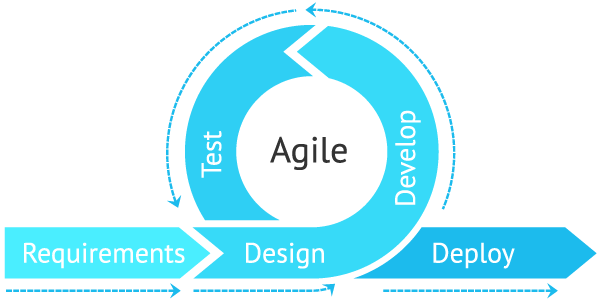
\includegraphics[width=0.6\linewidth]{images/methodology-agile.png}
    \end{center}
    \caption{Agile software development flowchart for a single sprint.}
    \label{fig:agile_flow}
\end{figure}

Agile comes in many flavours and frameworks for teams to follow such as Scrum, Lean software development and Kanban. However, they all seek to solve the problems which bottom-up uni-directional software development (called ``waterfall") failed to address. Agile incorporates feedback-driven revision into the development process which allows quick pivoting based on all manner of contingent circumstances such as changing requirements, fickle clients and unforeseen roadblocks.

Regardless of flavour, Agile development incorporates many improvements into the software development life cycle. The client is involved as an active member the development process and does not end up with a potentially nasty surprise at the end. Short development (called ``sprints'') cycles and tight, frequent deliverables reduce the effects of decision paralysis, trying to find a ``perfect'' implementation and excessive feature creep where developers think up of new additions as they develop, resulting in a product that is never delivered.

Within this project, a relaxed version of Agile will be implemented which caters for the limited meeting time for the team. Normal Agile development requires daily standups and feature ownership of individual developers. However, since this is a solo development project and meetings only occur weekly, a more reasonable arrangement is to set sprint goals for delivery and review in short cycles.

We therefore structure work into variable 2 or 1-week sprints. Each sprint will begin with a meeting, consisting of a progress update of work done in the previous week and review of improvement points. Important points of critique will be added to the backlog if they are actionable. A selection of tasks will then be selected from the backlog to serve as the priorities for the upcoming sprint, based on developer bandwidth for the week.

Ideally, if manpower and time constraints could be ignored, the project would require a front-end developer, a back-end and database engineer, an asset designer and a product manager in order to correctly execute the development of an app that correctly applies the principles of addictive app design. Unfortunately, the former 3 roles are squashed onto a single developer. This report will thus fully document in later sections the actions taken to account for this shortage and the compromised features that may have had to be pushed onto the backlog in favour of developing more urgent features.

\subsection{Continuous Integration \& Development}
Developers often break their own code. Facebook, one of the world's largest social media giants, is known for the quality of their engineers. Yet, one of their key tenets is ``Move fast, break things'', for fear of causing a malfunction in code is one of the largest inhibitors of progress. Yet, system downtime and app crashes often shake customer confidence in a product. DevOps practices under the Continuous Integration and Deployment (CI/ CD) umbrella refer to practices while automate and remove human error in the deployment and release process. Such practices include automated test runners built-in to version control, and automated tasks to build and test the product before automatically deploying it and releasing it to users.

Future developer manpower on this project will consist of a fluctuating student-manned team, each member of which may carry different levels of engineering competence. Implementing unopinionated DevOps infrastructure upfront therefore allows students to focus on developing and improving the customer-facing product without worrying about breaking the project, regardless of their level of engineering competence. Later sections will explore and detail the implementation of such infrastructure.

\section{Choosing A User-Interface Framework}
A long standing problem in the development of mobile applications has been that of having to maintain multiple codebases in order to increase user reach. Especially since different platforms almost always use completely different workflows and programming languages, this means having to employ multiple teams just to maintain separate codebases, leading to features being rolled out on one platform before another, or an inconsistent user experience between both platforms.

Cross-platform development seeks to solve this problem, often by creating a workflow in a given language which may then be transpiled into native platform code. While this solves the aforementioned problem, it also creates problems of its own. Cross-platform frameworks usually offer a reduced set of features compared to their native counterparts, since they effectively have to duplicate the API that the native platform exposes using different language semantics, which may not even be possible in some cases.

Despite this, cross-platform frameworks have found their niche in helping undermanned teams of developers bring a concept to market quickly. It is for this reason that this project will use a cross-platform framework in order to bring the product to iOS in a way that is extensible for future work, especially since no feature in this app requires the complexity that native development offers. The following subsections will evaluate the current two most popular choices of cross-platform frameworks.

\subsection{Flutter}
Flutter is a recent framework released in 2017 by Google, aiming to provide a set of out-of-the-box interface elements to enable quick development of beautiful user interfaces. As of the time of writing, Flutter has full support for iOS 14, Android 11, macOS, Windows and web \cite{fluttersupportedplatforms}.

However, the primary criticism of Flutter is not only its age, but that it runs in Dart, another language made by Google. This means that not as much libraries and packages for flutter are limited, which means likely having to write much more first-hand code and less stable releases of libraries.

\subsection{React Native}
React Native was released by Facebook in 2014 and continues to be one of the most developed open source projects on Github (alongside Flutter). It builds off of the Model-View-Update architecture originally implemented by React and shares many domain-specific semantics. It runs on JavaScript, which is by a large margin the world's most popular programming language \cite{sfdevsurvey} and therefore has full access to the open-source library distribution channels that it offers. This mean stable support on well-developed and community endorsed packages that enforce a standardised implementation of many common features that developers use.

The result is a smooth cross-platform experience that offers close-to-native performance and a fully-functioning native bridge to give developers full flexibility in writing native code where necessary. The success of React Native has attracted many reputable companies to build their platforms with it, such as Walmart, UberEats, Bloomberg and Pinterest \cite{rnplatforms}.

\subsection{Comparison}
The primary cause of concern regarding framework choice in this project is which one best enables speed of development. This project is scoped, designed and executed by a single engineer. The scope proposed so far is usually the work of multiple full-time software engineering teams. The age and reduced developer community size for Flutter is therefore a deal-breaker in this case. The NPM registry for JavaScript currently boasts over 1 million packages in comparison to its Flutter equivalent, pub.dev which currently has around 21000. Developer documentation and community FAQ pages are also likely to have answers to issues on JavaScript rather than Dart, which means much more time can be spent focusing on higher level application design instead of "re-inventing the wheel".

\section{Choosing a Cloud Hosting Vendor}
\subsection{Cloud Infrastructure}
Based on requirements so far, the application will also require a back-end with a database for persistent storage of user data. This, along with what will potentially be the web version of the app, will require hosting on a server. This section briefly evaluates a selection of popular cloud service vendors and how their offerings are relevant to the requirements of this project.

The offering of a Cloud-service provider can be thought of as the balance of two philosophies: "bare-metal" providers, and managed solutions. Bare-metal refers to the act of simply provisioning computing resources on a machine, the specifics of which are left up to the user to implement. The state-of-the-art nowadays would be for a developer to specify a containerised environment using a tool such as Docker or Kubernetes, effectively creating an isolated "container" which contains all the environmental requirements needed to run a desired program. A bare-metal service would then simply bill the developer based on pre-defined billing criteria such as CPU runtime, memory usage and network bandwidth consumption.

\begin{figure}[h]
    \begin{center}
        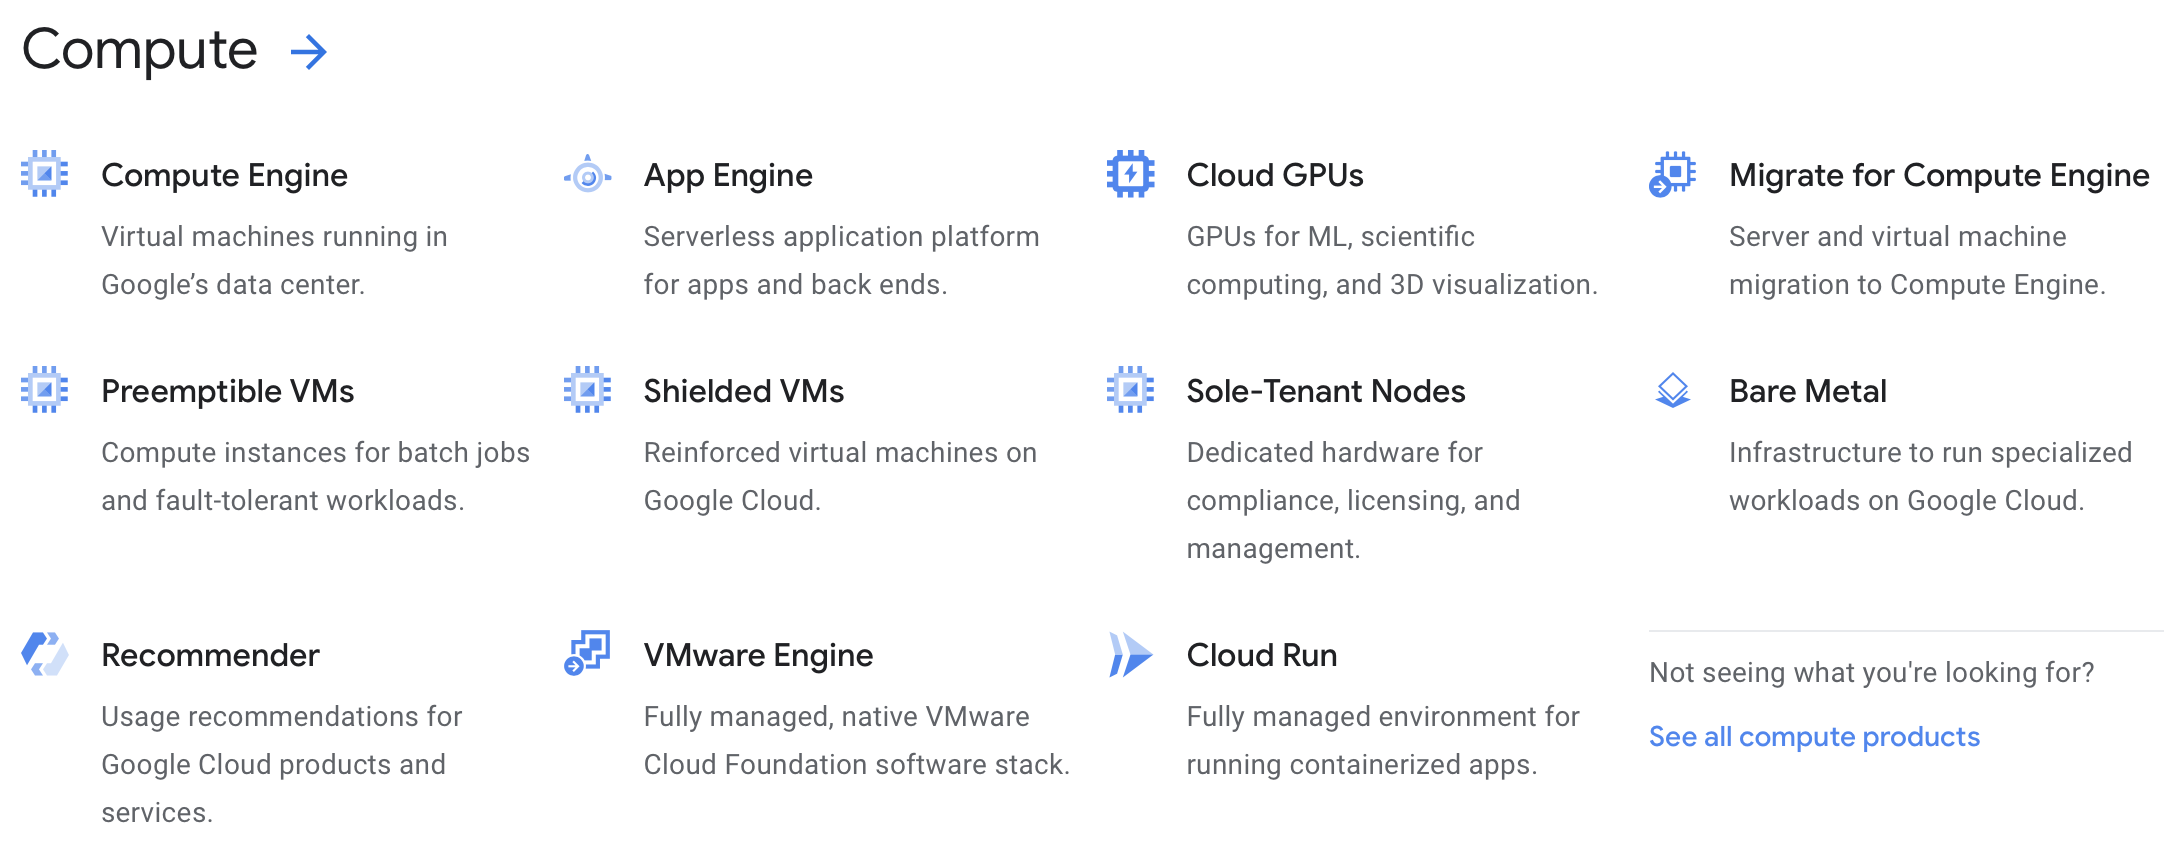
\includegraphics[scale=0.4]{images/google_cloud_compute_offerings.png}
    \end{center}
    \caption{Google Cloud compute product offerings}
    \label{gcp_compute_offerings}
\end{figure}

Managed solutions are built on top of the bare-metal philosophy. Cloud service providers may have specific offerings which deliver value to their customers in the form of pre-defined APIs which achieve a commonly desired functionality, such as user authentication. The market-leading solutions often provide a modular product selection that gives a developer a large degree of freedom to build suitable solution. One example of this is Google Cloud, which offers different degrees of control within its compute offerings, ranging from fully managed to completely bare metal. Solo-developer projects thus benefit greatly from the conveniences that managed workflows offer, and only employ bare-metal products where the flexibility offered is strictly necessary. In large enterprise teams, the reverse tends to be true, as maximal control over the codebase means less problems with software agility in the long run.

\subsection{Firebase}
Firebase began as a startup that was later acquired by Google and now stands as one of the most popular backend-as-a-service platforms for developers looking to get small projects off of the ground. Firebase currently offers an unparalleled out-of-the-box offering for implementing safe user authentication, identity management, database, on-demand cloud compute and many more essential features in a single workflow.

\begin{figure}[h]
    \begin{center}
        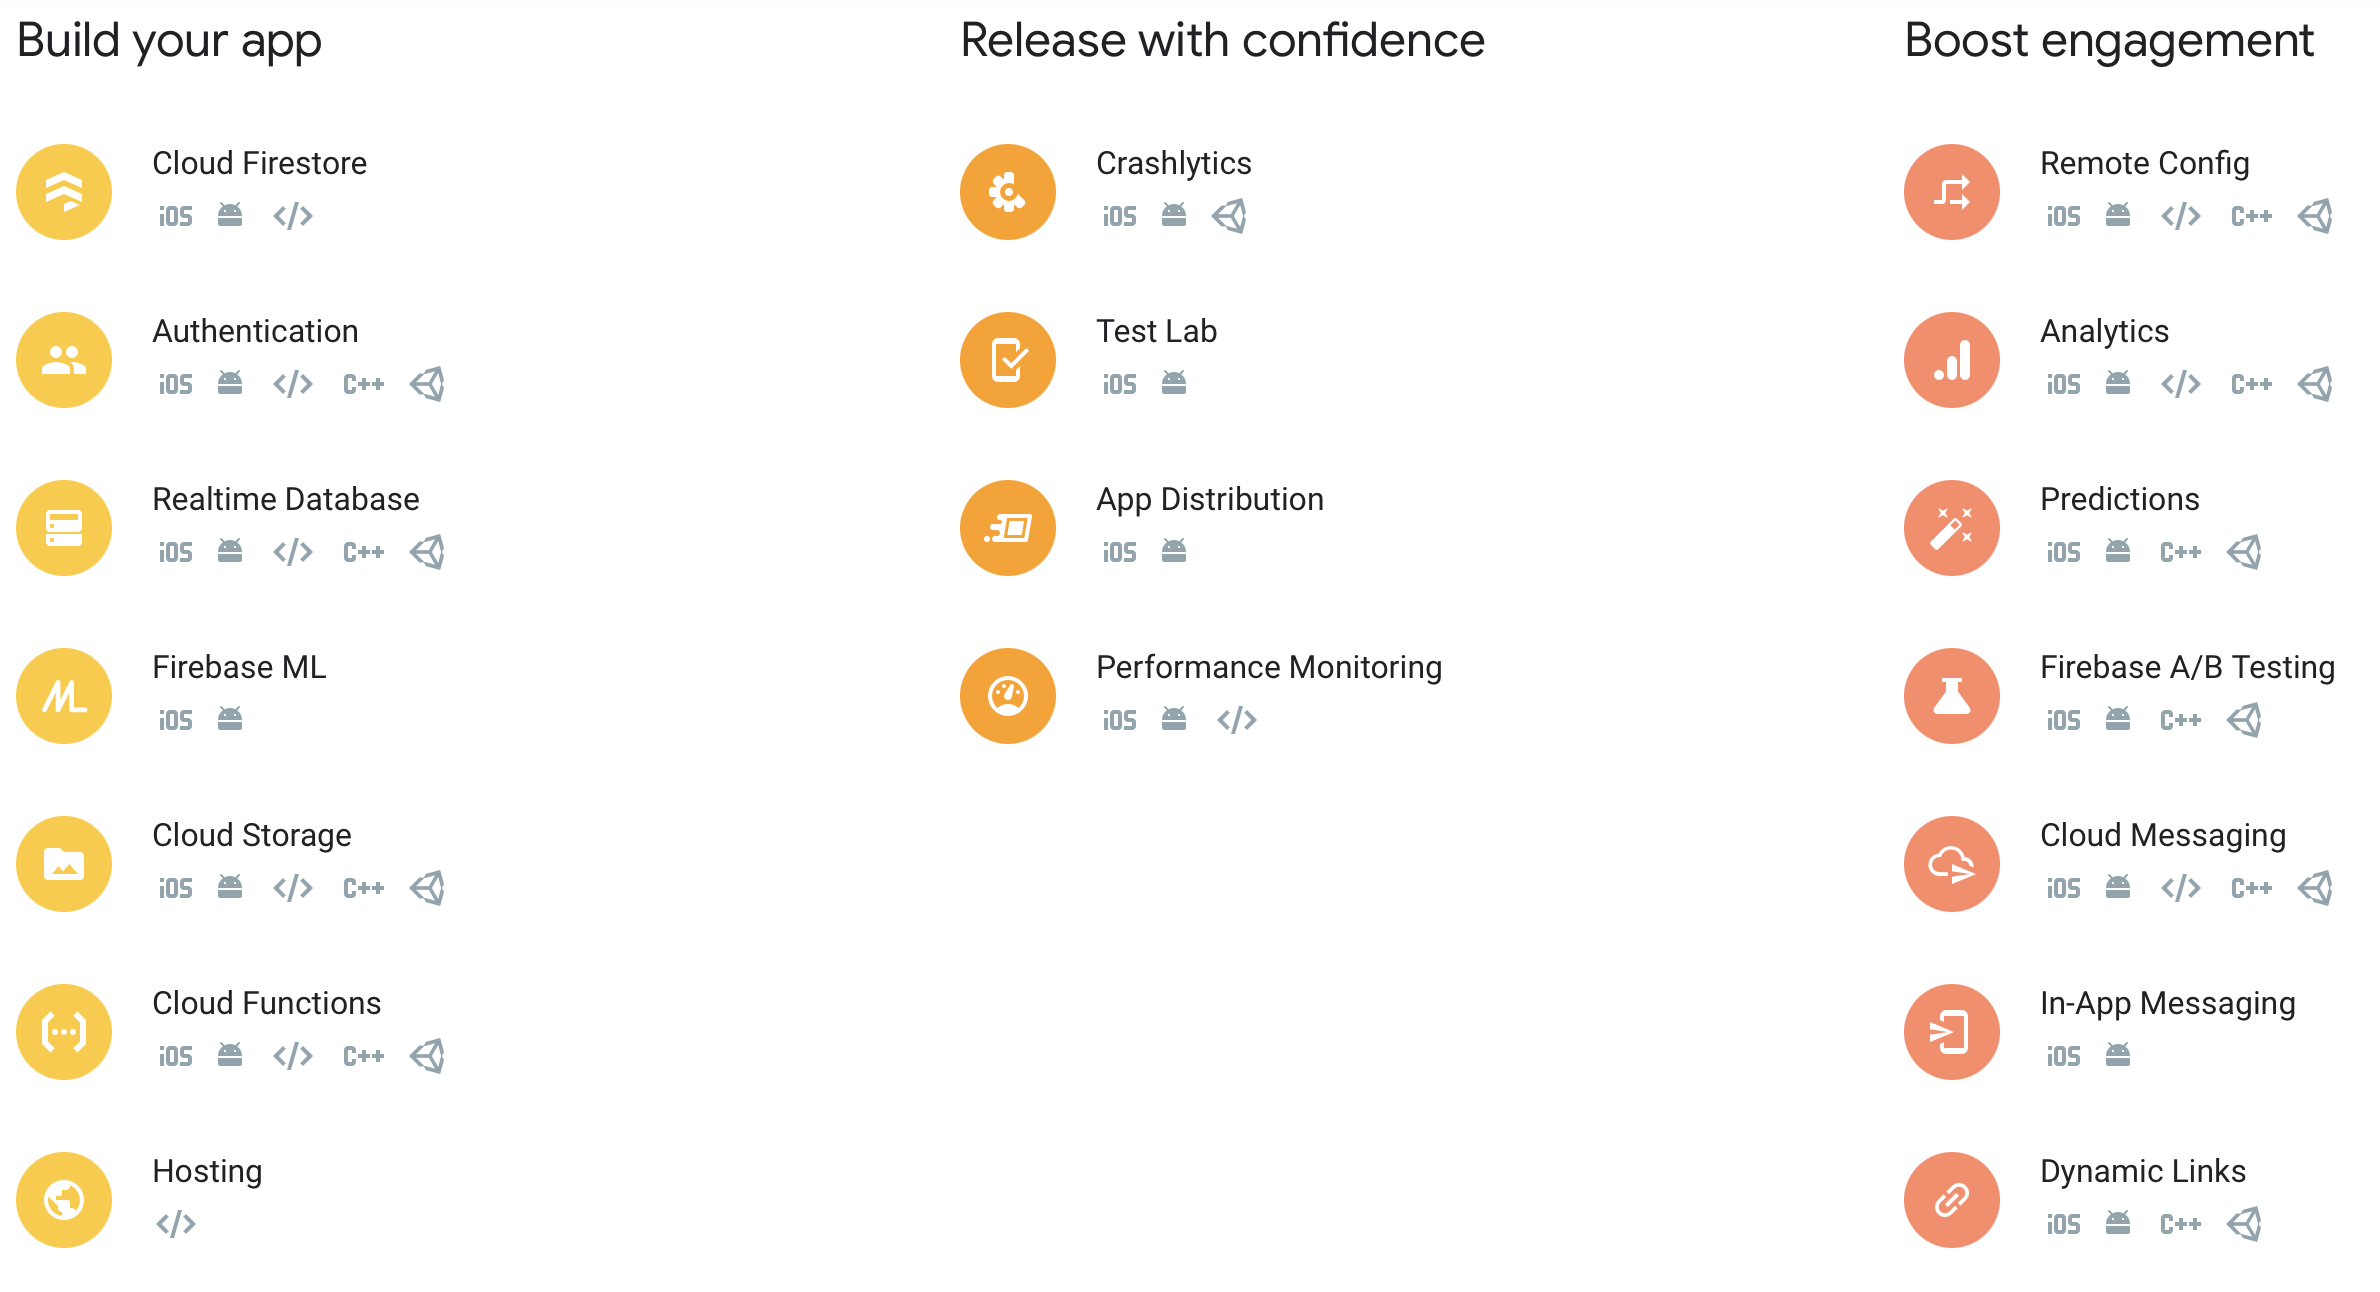
\includegraphics[scale=0.3]{images/firebase_offerings.png}
    \end{center}
    \caption{Firebase product offerings}
    \label{firebase_compute_offerings}
\end{figure}

However, all these benefits come at the cost: Firebase is closed-source and has vendor lock-in built into its design. Firebase is much more opinionated than the other back-end solutions that we have explored, in the following ways:

\begin{itemize}
    \item Databases are accessed directly by clients instead of a back-end endpoint through the Firestore or Realtime Database APIs.
    \item Firebase-provided databases are strictly non-relational (noSQL). Firebase offers no "bare-metal" products for developers to spin up their own databases using other paradigms.
    \item On-demand compute comes in the form of Firebase Cloud Functions, which is designed for small bursts of computation instead of long-running loops. The latter is still possible, but the resulting bill would be unfeasible.
    \item Cloud Functions currently only supports REST APIs and only supports a limited range of runtime environments.
\end{itemize}

Despite these, Firebase provides key functionality which may prove extremely valuable in continuing development for this project. Even if not implemented in this run of the project, Firebase offers out-of-the-box solutions for file storage, app crash analytics, search engine optimisation, A/B testing and even (limited) machine learning tasks. Therefore, it is undisputably the platform that will enable the fastest development of a workable product for this project.

In summary, the features that it provides will service the needs of future development on this project for a long time to come. Even if it should scale beyond that point, there should be enough resources to facilitate a migration away from Firebase anyway.

\section{Evaluation Plan}
Instead of the typical academic approach of conducting individual user studies on a select sample, this app hopes to build feedback in to the app as part of the user experience. The app is thus hosted on a cloud provider with a generous "free tier" allowance, allowing us to experiment with a sizeable user base of what we estimate to be up to 500 users before cloud computing costs actually start to kick in.

For this study, the concerns are not to develop the world's best-selling productivity app or to gain traction with a massive user base. This preliminary phase of the project is to find a way to measurably determine how effectively the Sage platform does its job of helping users stay on task. The refinement, re-selection and validity of these metrics will have to be determined as part of future work when the app is released in beta to the test audience. As an example, we may wish to measure a given user's productivity on a day-to-day basis by capturing a ``productive window'' in which a user continues to execute tasks without a significant (15 minute) disruption.

The app will be released to students in Imperial College London through the Android and iOS distribution channels, with its intentions clearly stated in both publicity efforts and as part of the in-app onboarding process. The goal is to complete development on the alpha release in time for the Easter holiday, when students will be focusing on studying for exams.

\section{Ethical, Legal and Safety Plan}
This project has no actionable safety concerns, since there is no physical product in which the user might harm themselves with. The primary concerns are with the use of third-party intellectual property and the safe and ethical use of user data for analytics and product improvement.

\subsection{Software Licensing}
This project will leverage the use of open-source software libraries and frameworks, the largest example of which is React Native. Open-source, by definition, allows the unrestricted redistribution and modification of a given piece of software for any purpose. As a secondary precaution, all packages used will be derived from the Node Package Manager (NPM) registry, which effectively serves as a central distribution point of open source packages pertaining to the javascript ecosystem (in which this project resides).

Most, if not all packages registered on NPM have an open-source approved license selected for their project. That is, a license which is in accordance with the open-source philosophy of freely useable, modifiable and shareable code. The list can be found at \href{https://opensource.org/licenses}{the open source initiative organisational website}. Should the exceptional case arise in which a package is used which does not use one of these licenses, it will be explicitly justified and disclosed in its implementation documentation. However, this should technically never arise.

\subsection{User Data Legal Compliance}
This study will use the General Data Protection Regulation (GDPR) as a basis of rules to follow in the ethical collection and use of user data. The following subsections will outline the parts of the GDPR deemed relevant to the nature of data used in this study, and perform a risk assessment of where grey areas may occur.

In the interest of brevity, the GDPR checklist can be found \href{https://gdpr.eu/checklist/}{here}. In addition to having completed this checklist, the Sage application will adopt the following policies for the collection of user data:

\begin{itemize}
    \item Once implemented, users will be explicitly informed via a transparent and detailed privacy policy what data we collect for evaluation metrics and how we will use it. The usage of the app requires the user to consent to this, as there is otherwise no point in offering the service which could otherwise incur cloud computing costs.
    \item The application does not capture any data defined by the GDPR as "personal", except for the user's email. Evaluation metrics, while potentially changing over the course of the project, should not allow the de-anonymisation of a given user.
    \item Data will be sent and stored using secure channels, using third-party GDPR compliant vendors where applicable.
    \item In the unlikely event of a data leak, users will be immediately informed via email what was leaked. However, none of this data should be particularly harmful to a user even if this should happen.
    \item Users may at any time erase all their usage data within the settings menu.
\end{itemize}

\section{Concluding Remarks}
A full implementation plan has been developed. However, the primary cause concern for this project is the shortage of developer manpower. Successful social media apps are usually developed across large enterprise teams, each of which ``owns'' a specific part of the product. Even then, a polished product typically emerges only after many cycles of product iteration. A realistic goal for this project is therefore to implement an excellent product to the best of our ability and have infrastructure in place to guide future development and iteration.
